\documentclass[journal,12pt,onecolumn]{IEEEtran}
\usepackage{cite}
 \usepackage{caption}
\usepackage{graphicx}
\usepackage{amsmath,amssymb,amsfonts,amsthm}
\usepackage{algorithmic}
\usepackage{graphicx}
\usepackage{textcomp}
\usepackage{xcolor}
\usepackage{txfonts}
\usepackage{listings}
\usepackage{enumitem}
\usepackage{mathtools}
\usepackage{gensymb}
\usepackage{comment}
\usepackage[breaklinks=true]{hyperref}
\usepackage{tkz-euclide} 
\usepackage{listings}
\usepackage{gvv}
%\def\inputGnumericTable{}                                 
\usepackage[latin1]{inputenc} 
\usetikzlibrary{arrows.meta, positioning}
\usepackage{xparse}
\usepackage{color}                                            
\usepackage{array}                                            
\usepackage{longtable}                                       
\usepackage{calc}                                             
\usepackage{multirow}
\usepackage{multicol}
\usepackage{hhline}                                           
\usepackage{ifthen}                                           
\usepackage{lscape}
\usepackage{tabularx}
\usepackage{array}
\usepackage{float}

\usepackage{float}
%\newcommand{\define}{\stackrel{\triangle}{=}}
\theoremstyle{remark}
\usepackage{circuitikz}
\captionsetup{justification=centering}
\usepackage{tikz}

\title{Matrices in Geometry 5.2.38}
\author{EE25BTECH11035 - Kushal B N}
\begin{document}
\vspace{3cm}
\maketitle
{\let\newpage\relax\maketitle}
\textbf{Question: }\\
Solve the following system of equations.\\
\begin{equation*}
\frac{1}{2x}+\frac{1}{3y} = 2
\end{equation*}
\begin{equation*}
    \frac{1}{3x}+\frac{1}{2y} = \frac{13}{6}
\end{equation*}

\textbf{Solution: }\\
Let

\begin{equation}
\vec{x} = \myvec{\frac{1}{x}\\ \frac{1}{y}}
\end{equation}

So that the given equations, after multiplying by 6 on both sides, can be represented in the matrix form as

\begin{equation}
    \myvec{3&2\\2&3}\vec{x} = \myvec{12\\13}
\end{equation}

Which can be represented as the augmented matrix
\begin{equation}
    \augvec{2}{1}{3&2&12\\2&3&13}
\end{equation}

\begin{equation}
    \augvec{2}{1}{3&2&12\\2&3&13} \xleftrightarrow{R_2 \leftarrow R_2 - \frac{2}{3}R_10} \augvec{2}{1}{3&2&12\\0&\frac{5}{3}&5}
\end{equation}

\begin{equation}
    \xleftrightarrow{R_1 \leftarrow R_1 - \frac{6}{5}R_2} \augvec{2}{1}{3&0&6\\0&\frac{5}{3}&5}
\end{equation}
So, by this, we get
\begin{equation}
    \frac{1}{y} = 3 \implies y = \frac{1}{3}
\end{equation}

\begin{equation}
    \frac{1}{x} = 2 \implies x = \frac{1}{2}
\end{equation}

\textbf{Final Answer: }\\
The solution for the given system of linear equations is $x = \frac{1}{2}$ and $y = \frac{1}{3}$.

\begin{figure}[H]
    \centering
    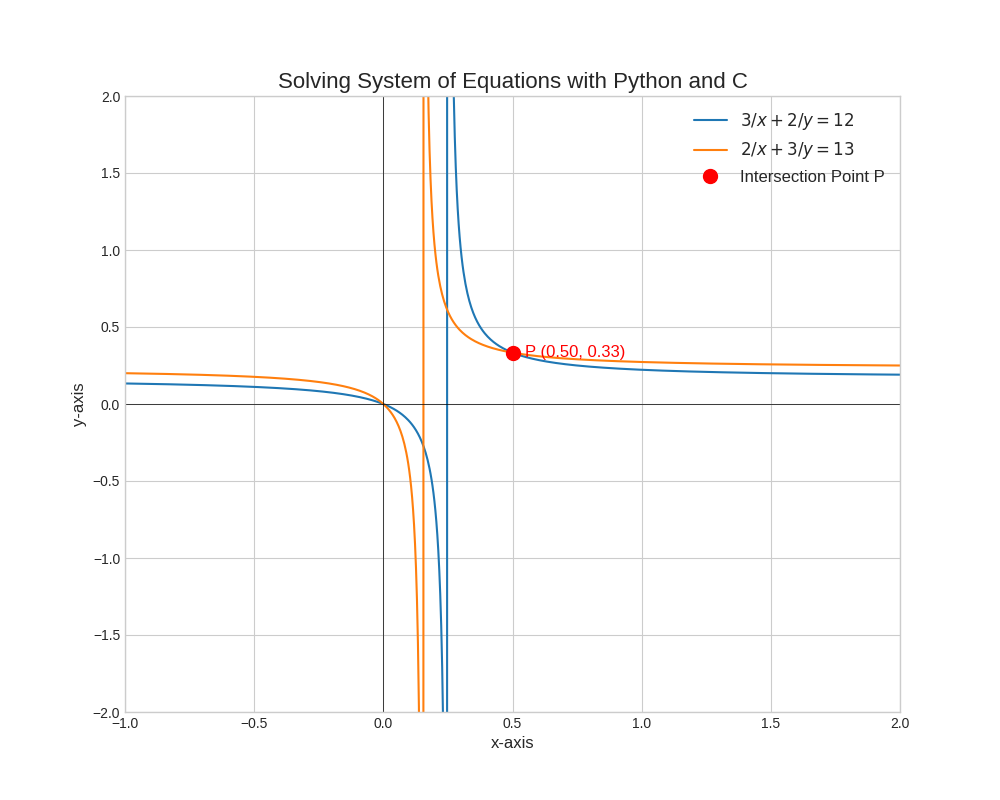
\includegraphics[width=0.75\columnwidth]{figs/1.png}
    \caption{}
\end{figure}

\end{document}